\section{Communication network}

Having functionality distributed across several instances sets the need for communication between the instances.
Based on Figure~\ref{fig:slave_structure}, which displays the dependency between \deno{B}, \deno{M}, and \deno{S} this leads to the diagram shown in Figure~\ref{fig:dataflow_diagrem}. \\


\begin{figure}[!h]
    \centering 
    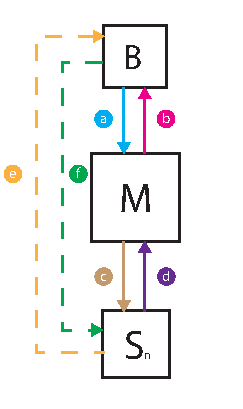
\includegraphics[width=0.5\textwidth]{gfx/dataflow_diagram.pdf}
    \caption{Dataflow diagram of \projectname{}}
    \label{fig:dataflow_diagrem}
\end{figure}


The arrows represent a connection, each connection represent dataflow in the direction of the arrow.
The type of data flowing in each connection and the reasons behind will be covered as each connection is discussed below. \\

Connection \deno{a} covers requests made by \deno{B}, which covers HTTP requests, which is a limit of web solutions that they must use the HTTP protocol.
HTTP requests enable the user to view the web application through his browser, and to send information.
In order to fulfill the request created by \deno{a}, a response is needed which the connection \deno{b} handles.
This connection covers the flow of the dynamic content created by \deno{M}, and static content such as: images, stylesheets, and multimedia objects.
Connection \deno{b} sends both the static and dynamic content back to \deno{B} to be displayed for the user. \\

The connection \deno{d} handles the signal described in Section~\ref{sec:functionality_distribution}.
This signal covers the initial communication between \deno{S} and \deno{M}. \deno{M} verifies the identity of \deno{S} by \deno{S} sending its own unique identifier.
This unique identifier is a string, which consist of X characters \fixme{How many chars?}.
All unique identifiers of each \deno{S} is known to \deno{M}.
This allows \deno{M} to determine the identity of each incoming signal. When \deno{M} receives a signal, and verify the identity of \deno{S}, the source location of the signal is stored in \deno{M} making \deno{M} able to know the location of \deno{S}. \\

Since requests from \deno{B} can happen asynchronously and from dynamic locations, it can create a problem that the identity of the connection made from \deno{S} to \deno{f} is not known. 
\at{28} sets the requirement of differentiating between incoming connections to \deno{S}.
If the communication described in connection \deno{e} and connection \deno{f} were running through \deno{M}, this would be no problem as security would be handled by the already existing sessions on \deno{M}.
The connections \deno{e} and \deno{f} are required to transport a large amount of data.
This data covers a video feed of the drone's video camera and commands for the drone.
This would increase the load on \deno{M}, which is not desired as \deno{M} is assumed to have a high load already.
However, since connection \deno{e} and connection \deno{f} are not running through \deno{M}, this leaves the problem of which \deno{B}, \deno{S} should listen to. \\

The solution chosen to solve this problem is to make \deno{S} create a randomly generated key (session key), that contains 40 characters and is unique relative to \deno{S} stored on \deno{S} itself.
When \deno{S} receives incoming commands, \deno{S} verifies whether or not the key received along with the command is equal to the one locally stored on \deno{S}.
If this is the case, \deno{S} classifies the received command as valid and performs the action.
The session key is delivered to \deno{B} from \deno{M}, as \deno{M} is able to verify the identity of \deno{B} through the session. \\

The connection \deno{c} covers requesting a session key by \deno{M}.
As \deno{M} has a static location, \deno{S} is able to verify the identity of \deno{M} based on its location.
Connection \deno{d} covers the response of the request received in \deno{c}, and \deno{M} is able to verify the identity of \deno{S} based on its location. \\

\begin{figure}[!h]
    \centering 
    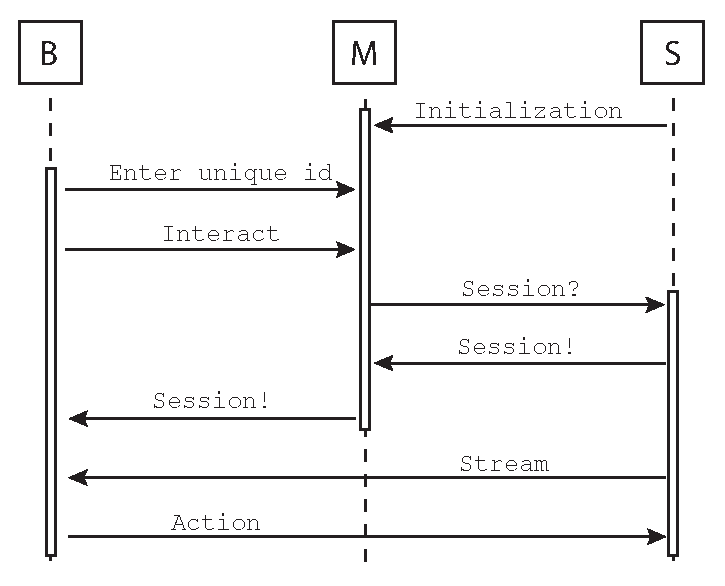
\includegraphics[width=\textwidth]{gfx/sequence_diagram.pdf}
    \caption{Sequence diagram of the communication network between \deno{B}, \deno{M}, and \deno{S}}
    \label{fig:sequence_diagram}
\end{figure}
\fxfatal{Sequence diagram: Activation boxes, or method-call boxes, are opaque rectangles drawn on top of lifelines to represent that processes are being performed in response to the message (ExecutionSpecifications in UML). I.e. its wrong at the moment.}


The functionalities of the described connections, can only happen in a sequence as illustrated in Figure~\ref{fig:sequence_diagram}.
Each message in the sequence diagram can be done multiple times, however above messages are enforced to be performed atleast once in order for the given message to be performed. \\


% The communication network is crucial for \projectname{} to work.
% When designing a scalable communication network it is important to choose the right structure.
% There are different ways when designing such a network but identical for them all is that they need to support the structure of \deno{M}, \deno{S} and \deno{B} described in section~\ref{sec:application_structure}.

% One solution is to make a structure where \deno{M}, \deno{S} and \deno{B} talk to each other with a level of security. 
% The security aspect would be implemented with a form of session key. 
% This key would be used to determine if a session between a \deno{B} and a \deno{S} is valid.
% Another solution is to provide no security aspect and let it be up to the users and / or company to keep drones safe from intruders.
% This would lessen the communication between \deno{B}, \deno{M} and \deno{S}.  
% It would also decrease the load on \deno{M} and \deno{S}'s database. 
% On the down side the system could be considered not safe because it would be possible to tamper with the drones.
% As this is a system where it is important that the integrity is high, evidence is not tampered with, and where the outcome of an unauthorized user controller a drone could be devastating, it is important to deliver some form of security.



% This lead to a solution where sessions is designed to keep the integrity and secure evidence as seen in figure~\ref{fig:sequence_diagram}. 
% As seen in the figure there is designed a level of security because of the sessions.
% It is not possible for a \deno{B} to interact with a drone without having a session with a drones \deno{S}.

% When a drone is purchased a \deno{S} is setup at the location where the drone is going to operate.
% The \deno{S} sends an initializing message to \deno{M}, informing \deno{M} that a new drone has entered the system.
% \deno{M} adds the drone with the IP and location of the \deno{S}, along with the drone's unique identifier.
% If \deno{M} receives an initializing message from a \deno{S} with a drone identifier that is already in the system, it will destroy any session that correlates with that drone.
% The sessions is destroyed because if one or more sessions are granted and \deno{S} sends its initializing message it is safe to assume that \deno{S} either disconnected or crashed and all sessions keys are invalid.
% Furthermore if the IP of \deno{S} differs from the IP \deno{M} holds in its database it will be updated.

% If a user tries to interact with a drone the system behaves differently.
% A session key will be made on a \deno{S}, this key will be send to \deno{M} and giving to \deno{B}. If this session key is valid it is possible for the user to communicate directly with \deno{S} without \deno{M}.

% \begin{figure}[!h]
%     \centering 
%     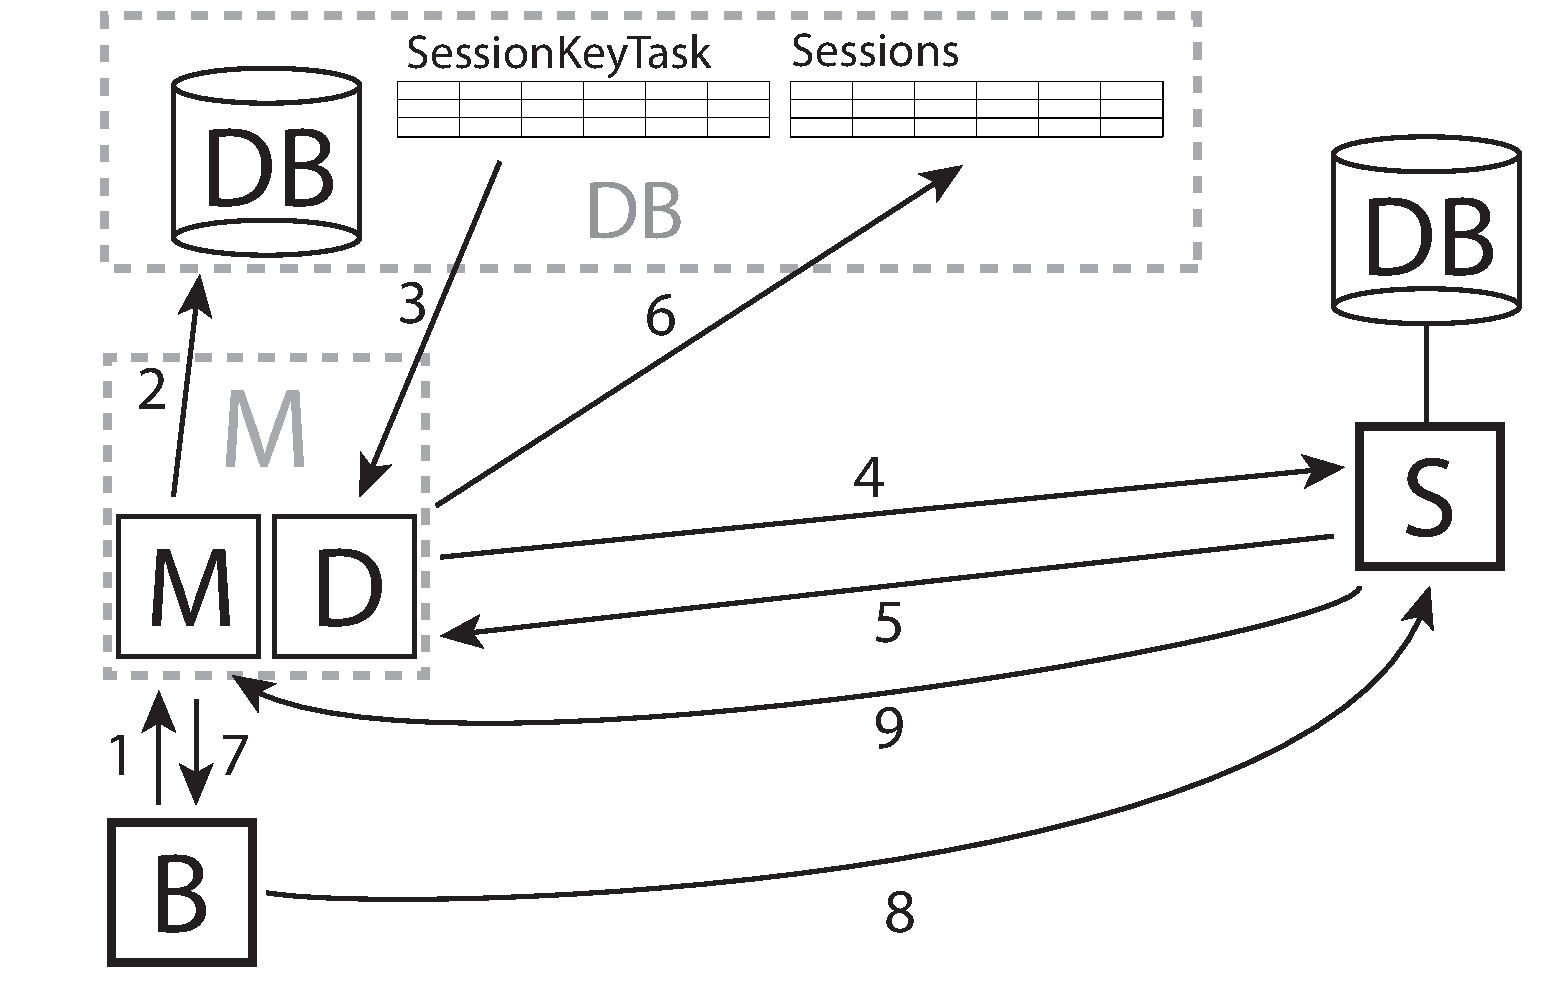
\includegraphics[width=\textwidth]{gfx/sessionkey_communication.pdf}
%     \caption{Session key communication between \deno{B}, \deno{M}, and \deno{S}}
%     \label{fig:sessionkey_communication}
% \end{figure}

% This behavior can be seen in figure~\ref{fig:sessionkey_communication}. 

% Session keys have been designed for security reasons.
% Firstly they were designed to ensure that only one user at a time can control a drone.
% Secondly it ensured that unauthorized users do not have the possibility of controlling a drone.

% \begin{enumerate}
% 	\item Request send from \deno{B} to \deno{M} about getting a session key to interact with a drone.
% 	\item \deno{M} inserts this request in its database table called SessionKeyTask.
% 	\item \deno{D} scans the database table SessionKeyTask, when it sees a new entry it select it and then deletes it from the table.
% 	\item \deno{D} requests a session key from \deno{S} parred with the drone the user wants to interact with.
% 	\item \deno{S} makes a random generated string with uppercase, lowercase letters and number. This string is used as the session key. \deno{S} updates its database with this session key and then sends it back to \deno{D} on \deno{M}.
% 	\item \deno{D} inserts the newly received session key into the session table of \deno{M}.
% 	\item \deno{M} then contacts \deno{B} with the session key.
% 	\item \deno{B} uses this session key to access \deno{S} and through it interact with the drone.
% 	\item A Timeout happens if \deno{B} and \deno{S} does not communicate for 10 seconds.
% \end{enumerate}

% Communication between the servers in the system is crucial. 
% Therefore it is important design a method or a set of methods handling the communication between them. 
% One method could be to make a service which handles all these requests on each server.
% The problem however is that using a single service might create a bottleneck.
% An alternative solution is to make a service for each communication level.
% One service that handles sessions, a service that handles control commands, and a service that handles initial messages from \deno{S} see section~\ref{sec:application_structure}.\fxfatal{Den her paragraf er uspecifik}

% This lead to a solution where the different actors in the system delivered and / or depended on services.

% The interface of the communication network can be seen in figure~\ref{fig:communication_network}.

% The communication network of \projectname{} uses four different ports for providing its services:

% \begin{itemize}
% 	\item Port A - service port for sending and receiving drone control commands.
% 	\item Port B - service port for receiving and sending initial messages.
% 	\item Port C - service port for sending and receiving session information including session keys.
% 	\item Port Web - service port for sending and receiving web specific information.
% \end{itemize}

% \begin{figure}[!h]
%     \centering 
%     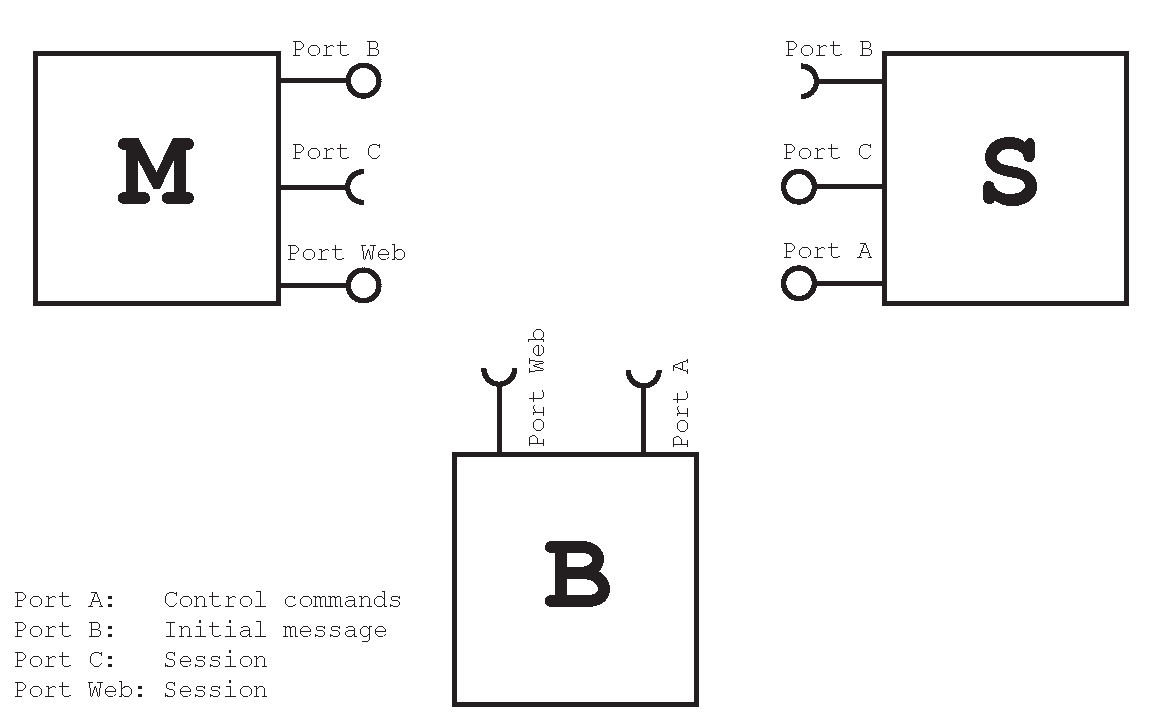
\includegraphics[width=\textwidth]{gfx/communication_network.pdf}
%     \caption{Communication network between \deno{B}, \deno{M}, and \deno{S}}
%     \label{fig:communication_network}
% \end{figure}

% When designing a communication network it is also important to select the right technique for exchanging data between services.
% One of the more widely used techniques are Extensible Markup Language.
% Extensible Markup Language, or XML for short, is a markup language designed to easily mark up data.
% The markup that XML provides makes it possible to easily send and receive data.
% The Extensible in XML makes it possible to extent what data types XML can handle through the XML schema. \citep{simonstl}
% This gives XML a drawback because XML is designed to be extensible it also carries a lot of overhead when used to mark up data.

% \projectname{} needs to be scalable therefore it is important to use as little overhead when sending structured information.
% Otherwise there is a chance that this overhead creates a bottleneck within the network.

% JSON, or JavaScript Object Notation, is design for data interchange and to be human-readable.
% It have a simpler syntax than XML and is not build to be extensible, it is not even a markup language. 
% It is a structured way of exchanging data between sources. 
% This results in less overhead i.e. it costs less data for each piece of information. 
% JSON is also data orientated which makes it easier to map a JSON object directly to a object orientated structure.
% Douglas Crockford call JSON ``The Fat-Free Alternative to XML'' \citep{JSON}.

% Therefore JSON is the perfect format for data interchange between the different services in \projectname{}. There are lesser costs associated with JSON than XML and it is easier to map them into a object orientated language.